\section{Matrices: array of numbers}

%Lecture 9.11




Matrices are rectangular arrays of numbers:

$$
A = 
\left[
\begin{matrix}
a_{11} & a_{12} & ... & a_{1n} \\
a_{21} & a_{22} & ... & a_{2n} \\
... & ... & ... & ...\\
a_{m1} & a_{m2} & ... & a_{mn}
\end{matrix}
\right] \in \reals^{m\times n}
$$


The element in the $i^{th}$ row \& $j^{th}$ column: $a_{ij} = [A]_{ij}$(equivalent notation)

The transposition operation works on matrices by exchanging rows and columns: 
$$
A^T = 
\left[
\begin{matrix}
a_{11} & a_{21} & ... & a_{1n} \\
a_{12} & a_{22} & ... & a_{m2} \\
... & ... & ... & ...\\
a_{1n} & a_{2n} & ... & a_{mn}
\end{matrix}
\right] \in \reals^{m\times n}
$$

So $[A]_{ij}  = [A^T]_{ji}$ if $A\in \reals^{m\times n}$ then $A^T\in \reals^{n\times m}$

Operations of matrices:

1) $A + B = C$,  where $[C] = [A]_{ij} + [B]_{ij}$

2) $\alpha A = B$, where $[B]_{ij} = \alpha [A]_{ij}$

Note: the origin is a all-zero matrix. 


\begin{definition}{\textbf{Inner product of matrices}} 
	
	Let $A, B\in\reals^{m\times n}$, the inner product of metrics $A$ and $B$ is defined as
		$$\langle A, B\rangle = \text{trace}(A^TB) = \text{trace}(BA^T)$$ 
		where $A^TB\in \reals^{n\times n}$ and $B^TA\in \reals^{m\times m}$, and the trace($X$) for a given matrix $X$ is defined as the sum of the diagonal elements of $X$.
\end{definition}



\textbf{Length of Matrix: Norm}

We introduce the Frobenius norm here but note that there are also other matrix norms(e.g., spectrum norm, nuclear norm)

Frobenius Norm: 

$$\Vert A\Vert _F = \sqrt{<A, A>} = \sqrt{\text{trace}(A^TA)} = \sqrt{\sum^m_{i=1}\sum^m_{j=1}[A]^2_{ij}}$$


%$$\vec{(A)} = \text{vec}
%\left(
%\left[
%\begin{matrix}
%... & ... & ... & ... \\
%a_{1} & a_{2} & ... & a_{n} \\
%... & ... & ... & ...
%\end{matrix}
%\right]\right) = 
%\left[
%\begin{matrix}
%a_{1} \\
%a_{2} \\
%... \\
%a_{n}
%\end{matrix}
%\right]
%\in \reals^{m\times n}
%$$


\textbf{Matrix inverse}

An $n$ by $n$ matrix $A$ is called "invertible", if $\exists$ unique $A^{-1}$ s.t. $AA^{-1} = A^{-1}A = I$. The matrix $A^{-1}$ is called the inverse of matrix $A$\\

\vspace{0.3cm}
Some properties for invertible matrices:
\begin{itemize}
	\item $(AB)^{-1} = B^{-1}A^{-1}$, where $A, B\in\reals^{n\times n}$
	\item $(A^{-1})^T = (A^T)^{-1}$
	\item $\det(A^{-1}) = \frac{1}{\det(A)}$
\end{itemize}

Now, thinking the matrix $A_{m\times n}$ as a mapping, i.e., $A:\reals^{n}\mapsto\reals^{m}$ (or sometimes denotes as $F:\reals^{n}\mapsto\reals^{m}$, where $F$ is a linear mapping), the inverse of A might thinking as a inverse of the original mapping, that is, map $\reals^{m}$ back to $\reals^{n}$. The question remains is how to achieve this. 

Notice that:

(1) If $m<n$ , it is impossible to map $\reals^{m}$ back to $\reals^{n}$.

(2) If $m\geq n$, it is possible to achieve this inverse mapping.

Remark: There is a thing called "pseudo inverse" for non square matrix.



\subsection{Matrices as linear \& affine maps}
A map $F:\cal{V}\mapsto\cal{W}$ is "linear if for any two points $x^{(1)}, x^{(2)}\in\cal{U}$ and scalar $a_1$ and $a_2$ have
$$F(a_1 x^{(1)} + a_2 x^{(2)}) = a_1 F(x^{(1)}) + a_2 F(x^{(2)})$$

It turns out that any linear map is completely specified by a matrix. For example, back to basic linear system, $Ax=y$, the linear mapping maps $x\in\reals^n$ to $y\in\reals^m$, via the multiplication of matrix $A$.

Furthermore, affine maps are linear functions plus the offset, i.e., $F(x) = Ax + b$ where $A\in \reals^{m,n}$, $b\in \reals^m$




\subsection{Approximations}


Recall that previously we have talked about approximation of a function $F:\reals^{n}\mapsto\reals$, and now we are going to consider the case $F:\reals^{n}\mapsto\reals^m$.


A nonlinear map $F: \reals^n \rightarrow \reals^m$ can be approximated by an affine map(so we are considering a stack of functions now):
\begin{align*}
F(x)&=\begin{bmatrix}
F_1(x)\\
F_2(x)\\
\vdots\\
F_m(x)\\
\end{bmatrix}\\
&=
\begin{bmatrix}
F_1(x_0)\\
F_2(x_0)\\
\vdots\\
F_m(x_0)\\
\end{bmatrix}
+
\begin{bmatrix}
\nabla F_1(x_0)^\trans\\
\nabla F_2(x_0)^\trans\\
\vdots\\
\nabla F_m(x_0)^\trans\\
\end{bmatrix}
(x-x_0)
+
o(\Vert x - x_0\Vert)\\
&=
\begin{bmatrix}
F_1(x_0)\\
F_2(x_0)\\
\vdots\\
F_m(x_0)\\
\end{bmatrix}
+
\begin{bmatrix}
\frac{\partial F_1(x_0)}{\partial x_1}&\cdots&\frac{\partial F_1(x_0)}{\partial x_n}\\
\vdots& &\vdots\\
\frac{\partial F_m(x_0)}{\partial x_1}&\cdots&\frac{\partial F_m(x_0)}{\partial x_n}
\end{bmatrix}
(x-x_0)
+
o(\Vert x - x_0\Vert)\\
&= F(x_0) + J_F(x_0)(x - x_0) + o(\Vert x - x_0\Vert)
\end{align*}

where $o(\Vert x - x_0\Vert)$ are terms that go to zero faster than 1st order for $x\rightarrow x_0$ and $J_F(x_0)$ is the Jacobian of $F$ evaluated at $x_0$:

$$J_F(x_0) = 
\left[
\begin{matrix}
\frac{\sigma f_1}{\sigma x_1} &  ... & \frac{\sigma f_1}{\sigma x_n} \\
... &  ... & ...\\
\frac{\sigma f_m}{\sigma x_1} &  ... &\frac{\sigma f_m}{\sigma x_n}
\end{matrix}
\right]_{x = x_0}
$$

For $x$ 'near' to $x_0$, the variation $\delta_F(x) =F(x) - F(x_0)$ can be approximated described by a linear map:
$$\delta_F(x) = J_F(x_0)\delta_x, \,\, \delta_x = x - x_0$$

\subsection{Orthogonal Matrices}

\begin{definition}
	$U\in \reals^{n\times m}$ is \textbf{orthogonal} if $U = [U^{(1)} ... U^{(n)}]$
	and 
	
	$$ U^{(i)^T}U^{(j)}=\left\{
	\begin{aligned}
	0\quad \forall i\neq j\\
	1\quad \text{if } i = j
	\end{aligned}
	\right.
	$$
\end{definition}

Then $UU^T = U^TU = I$\\

Next, let's see how orthogonal transformation do to geometry, i.e., to length and angles between vectors. Let $U$ be an $n$ by $n$ orthogonal matrix which defines a linear map from $x\in\reals^{n}$ to $y\in\reals^{n}$, that is, $y= Ux$.

(a) Length between vectors
$$\Vert y\Vert^2 = (Ux)^T(Ux) = x^TU^TUx = x^Tx = \Vert x\Vert^2$$


(b) Angle between vectors

To compare the angles between vectors, we consider two maps now, i.e., $v= Uw$ and $y= Ux$.
$$\langle y, v\rangle = \langle Ux, Uw\rangle = x^TU^TUw = x^Tw = \langle x, w\rangle$$

To summarize, the length of a vector and the angle between two vectors remain the same after an orthogonal transformation.



\subsection{Range, rank and null space}

Let's consider a linear map that $F:x\mapsto Ax$, where $x\in\reals^{n}$ and $A$ is $m$ by $n$ matrix.

Some important terminology regarding this map are illustrated as follows:

\begin{itemize}
	\item Domain
\end{itemize}

$\text{dom}(A)$ = $\reals^n$, $A = [a^{(1)}...a^{(n)}]$

$\text{dom}(A^T)$ = $\reals^m$, $A^T = [a^{(1)}...a^{(m)}]$


\begin{itemize}
	\item Range(or, Column space)
\end{itemize}

Range of $A$ is the set of vectors $y$ obtained as a linear combination of vectors $x\in \reals^n$, and takes the form $y= Ax$.

\begin{equation*}
R(A) = \{y\in \reals^m | y = Ax = \sum^n_{i=1}x_ia^{(i)}\}
\end{equation*}

\begin{equation*}
R(A^T) = \{w\in \reals^m | w = A^Tu = \sum^m_{i=1}u_ia^{(i)}\}
\end{equation*}

\begin{itemize}
	\item Rank
\end{itemize}

The dimension of the range of $A$ is called the rank of $A$:

\begin{equation*}
\rank(A) = \text{dim}\{R(A)\} = \text{dim}\{R(A^T)\} =\rank(A^T)
\end{equation*}

\begin{itemize}
	\item Nullspace (or, Kernel)
\end{itemize}

The nullspace of the matrix $A$ is the set of vectors in the input space that are mapped to zero vector:

\begin{equation*}
N(A) = \{x\in \reals^n | Ax = 0\}
\end{equation*}

\begin{itemize}
	\item Fundamental Theorem
\end{itemize}

We can find that for any $x\in R(A^T)$ and any $z\in N(A)$, it holds that $x^Tz = 0$.\\

$\reals^n = R(A^T) \bigoplus N(A)$: $\forall x\in \reals^n$ there is a unique $x = x_{R(A^T)} = x_{N(A)}$.\\

\begin{theorem}{Fundamental theorem of linear algebra}
	
	For any given matrix $A\in \reals^{m,n}$, it holds that $N(A) \perp R(A^T)$ and $R(A) \perp N(A^T)$, hence
	\begin{align*}
	\text{N}(A) \bigoplus \text{R}(A^T) &= \reals^n\\
	\text{R}(A) \bigoplus \text{N}(A^T) &= \reals^m\\
	\text{dim} \text{N}(A) + \rank(A) &=n\\
	\text{dim} \text{N}(A^T) + \rank(A) &=m
	\end{align*}
\end{theorem}

Consequently, we can decompose $\forall x\in \reals^n$ as the sum of 2 vectors orthogonal to each other, one in the range of $A^T$ and the other one is in the nullspace of $A$, i.e.,
$$x = A^T\xi + z,\ \text{where}\ z\in \text{N}(A)$$




\subsection{PageRank}

%Lecture Sep 16

PageRank algorithm: More important web page should be ranked higher


A page's important score can be interpreted as the number of “votes” that a page has received from other pages(or, the sum of importance score received from all its neighbors), and also a page can make a vote to other pages as well. Further more, if one page has made multiple votes to the others, then each vote it made is scaled by its total vote.

Therefore, the importance score of a page(or node) $i$ can be written as:
$$\pi(i)=\sum_{j \rightarrow i}\frac{\pi_j}{O_j}$$
where $j \rightarrow i$ means the set of all the neighbors(denote each neighbor as $j$) of $i$.

Let's consider following example
\begin{figure}
	\centering
	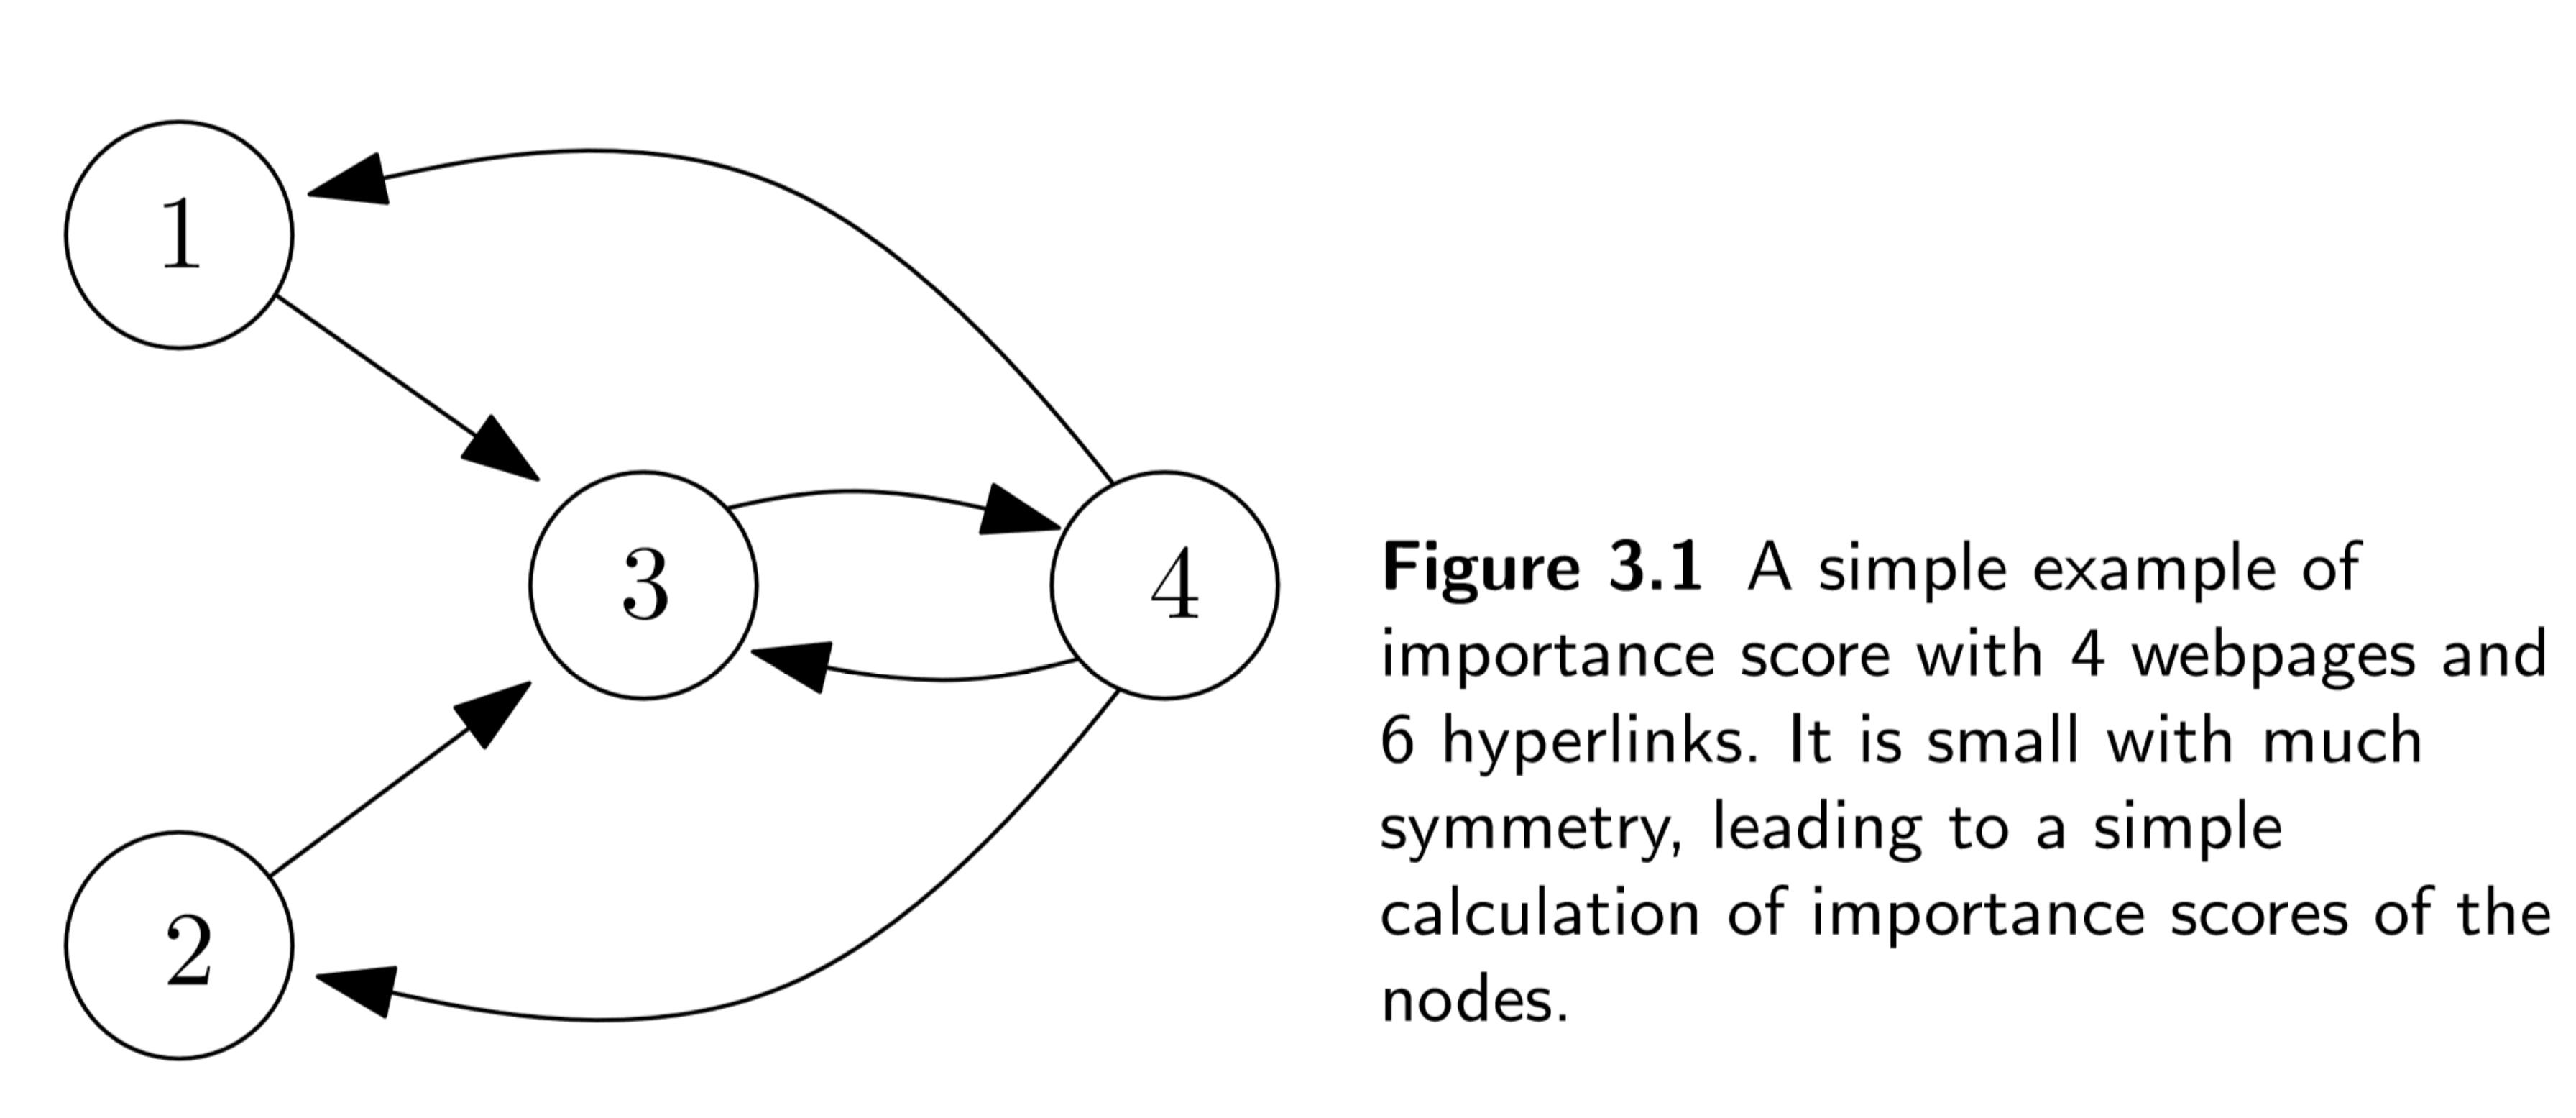
\includegraphics[width=2.1in,height=2.1in]{figures/ch03/figure0.jpg}
	%\caption{This is an inserted JPG graphic} 
	%\label{fig:graph} 
\end{figure}


Let the score of node 1 be x, and that of node 4 be y. Looking at node 1's incoming links, we see that there is only one such link, coming from node 4 that points to three nodes. So $x = \frac{y}{3}$ and $2x + 2y = 1$. The second equality comes from the normalization of importance scores, and it turns out node 1 and node 2 has the same importance score, and also node 3 and 4 have the same one as well. So the set of importance scores turns out to be [0.125, 0.125, 0.375, 0.375]. 

Let's define following terminology:

Matrix $H$: its $(i,j)$th entry is $\frac{1}{O_i}$ if there is a hyperlink from webpage $i$ to webpage $j$, and $0$ otherwise.

$\pi$: $N \times$1 column vector denoting the importance scores of the $N$ web pages.

Multiply $\pi^T$ on the right by matrix $H$, this is spreading the importance score from the last iteration evenly among the outgoing links, and re-calculating the importance score of each webpage in this iteration by summing up the importance scores from the incoming links. That is
$$\pi^T[k] = \pi^T[k - 1]H$$


%Note: $\pi^T[k] = \pi^T[k - 1]G$

When $k$ takes a large number(take a large number of iterations), we have the limiting distribution $\pi^{*\trans}$ for all the pages,
$$\pi^{*T} = \pi^{*T}H$$
Obviously, $\pi^{*T}$ is the left eigenvector of $H$ corresponding to the eigenvalue of 1.


Let's take a look in this example. For a graph like this:

\begin{figure}
	\centering
	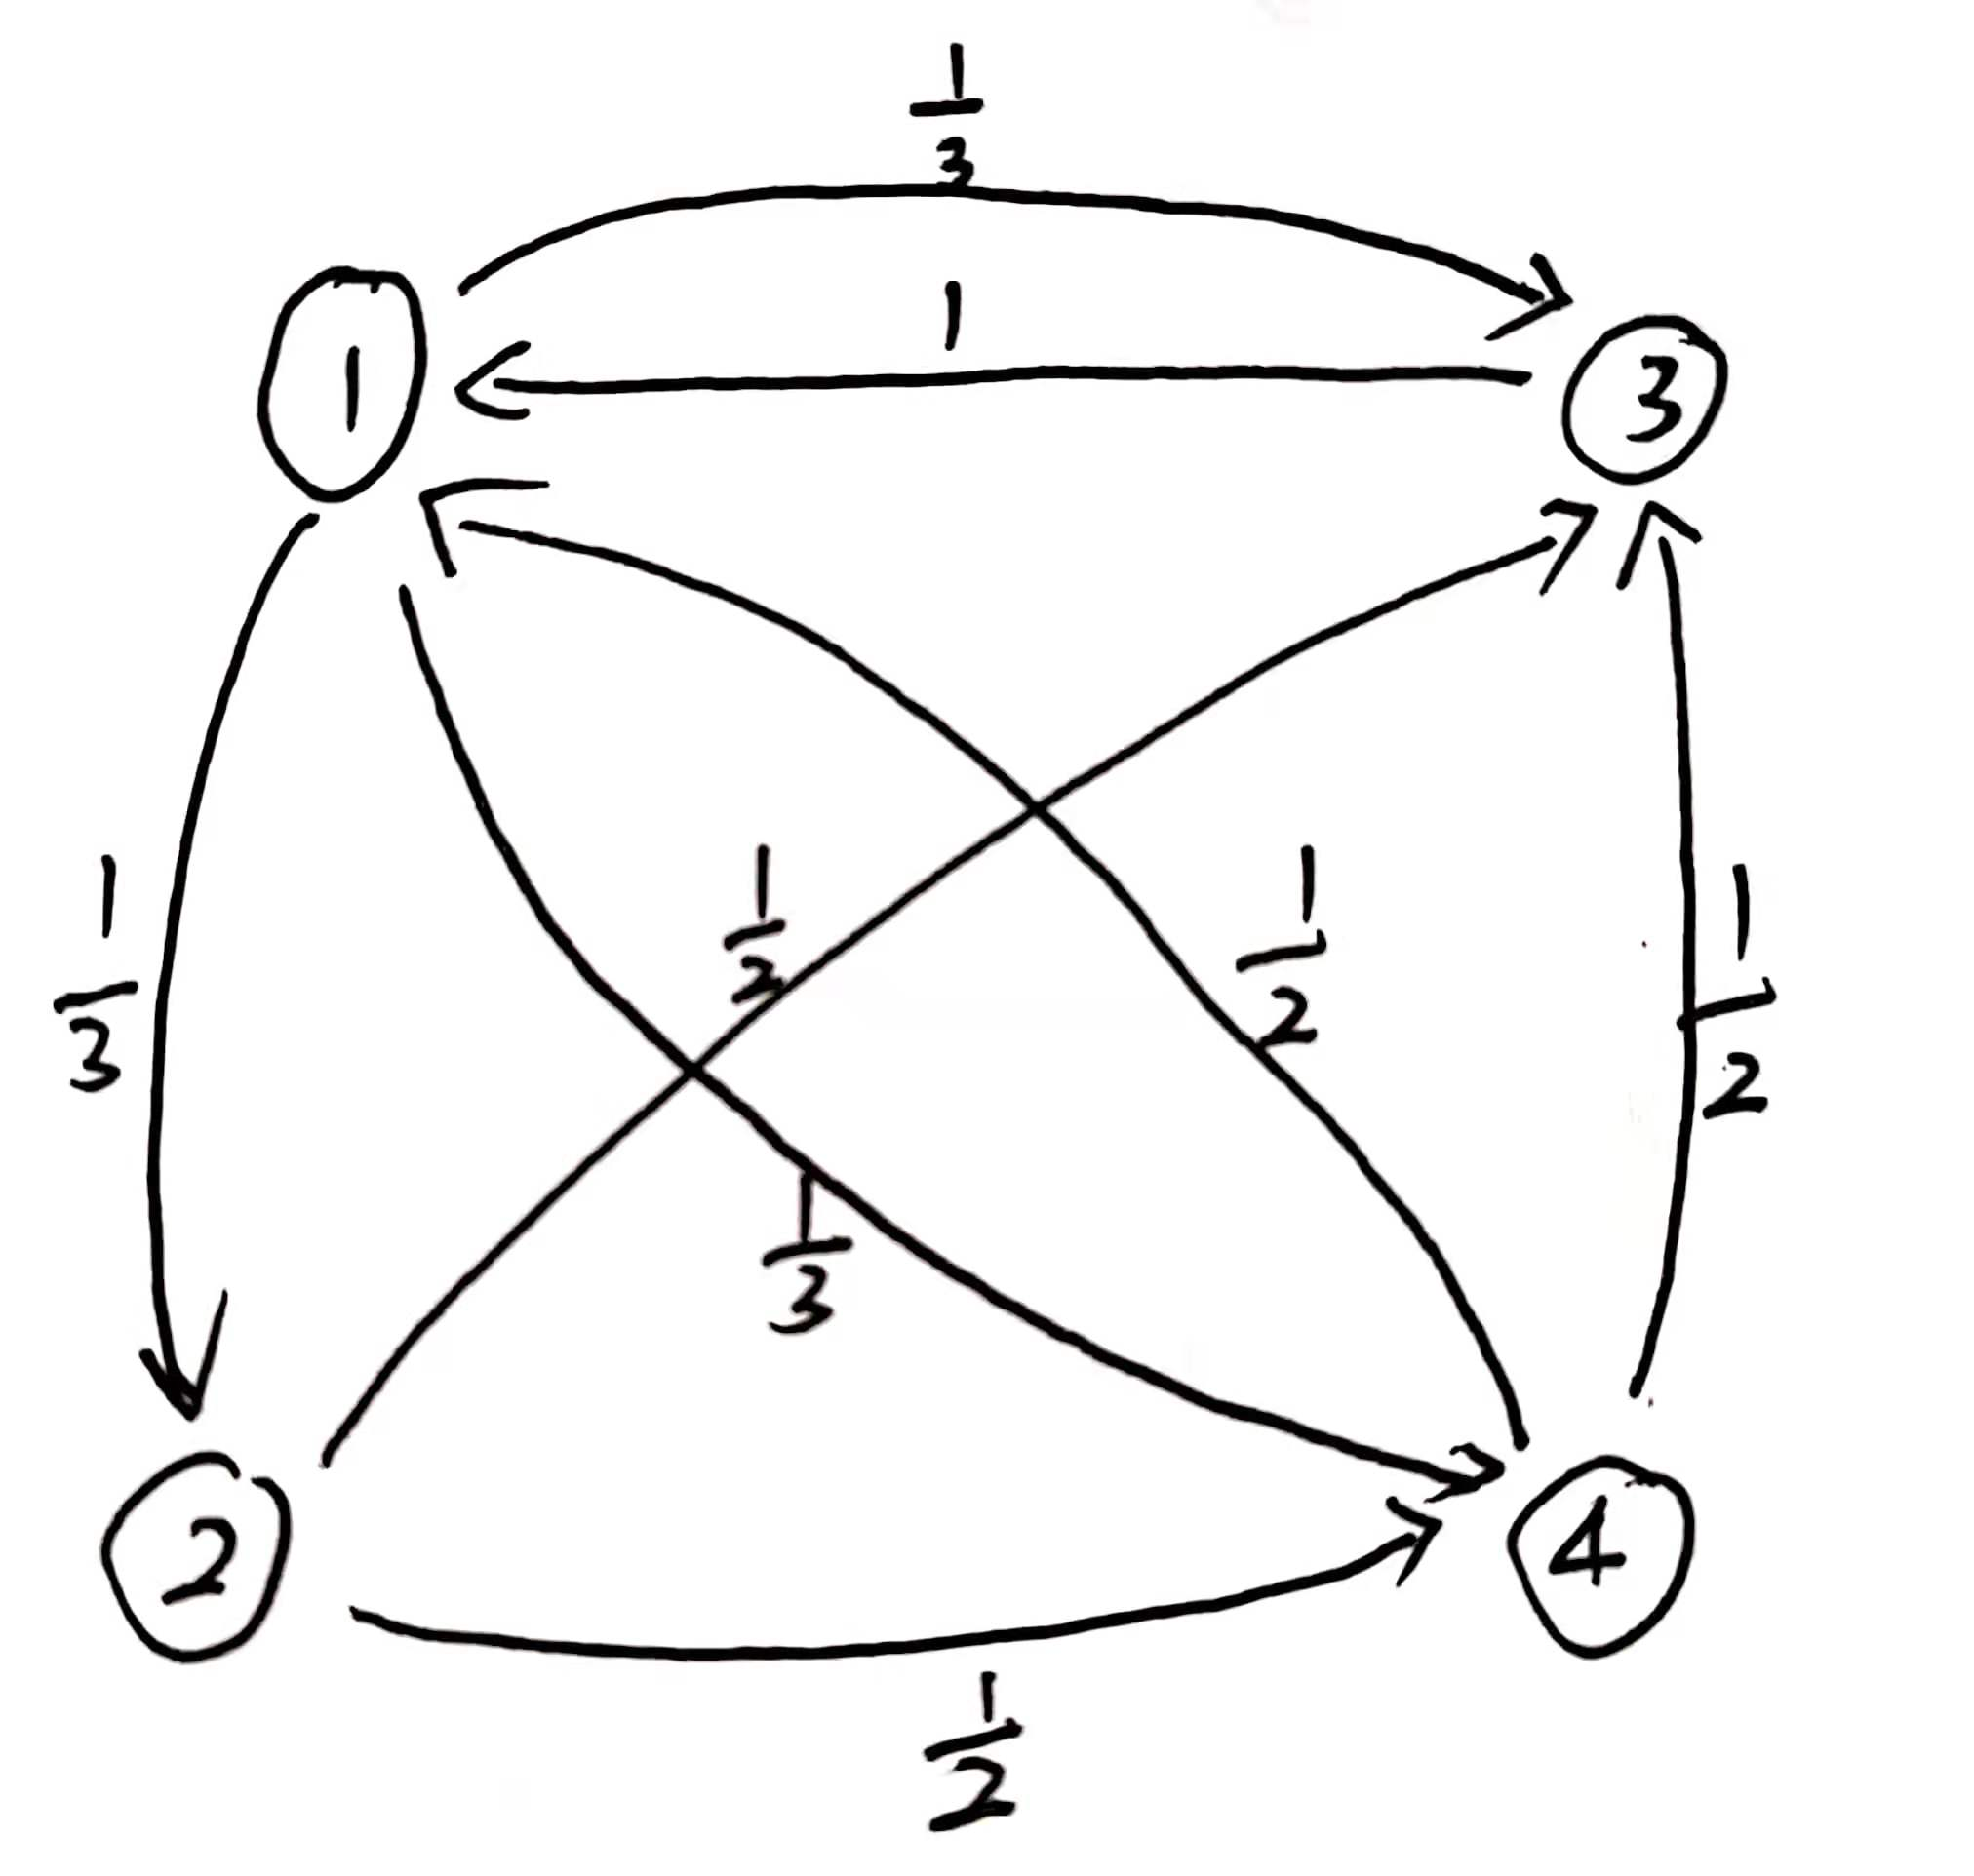
\includegraphics[width=2.1in,height=2.1in]{figures/ch03/figure3.jpg}
	%\caption{This is an inserted JPG graphic} 
	%\label{fig:graph} 
\end{figure}

$$
\left[
\begin{matrix}
x_1 \\
x_2 \\
x_3\\
x_4\\
\end{matrix}
\right] =
\left[
\begin{matrix}
0 & 0 & 1 & \frac{1}{2} \\
\frac{1}{3} & 0 & 0& 0 \\
\frac{1}{3}& \frac{1}{2} & 0 & \frac{1}{2} \\
\frac{1}{3} & \frac{1}{2} & 0 & 0 
\end{matrix}
\right]
\left[
\begin{matrix}
x_1 \\
x_2 \\
x_3\\
x_4\\
\end{matrix}
\right]
$$

The importance scores for each page can be computed as follows

\begin{align*}
x &= Ax \\
Ax - x &= 0\\
(A - I)x &= 0\\
x&\in N(A-I)
\end{align*}


$$
x = \frac{1}{s_1}
\left[
\begin{matrix}
12 \\
4 \\
9\\
6\\
\end{matrix}
\right]
$$
Note: 

\begin{itemize}
	\item $x^{(0)}$ is the initial distribution.
	
	\item $x^{(0)}_i = $Pr[start on page $i$]
	
	\item $u^{(i)}, \lambda_i$ is eigen-vector/value pair if $Au^{(i)} = \lambda_iu^{(i)}$, and we arrange this eigenvalues in a decreasing order from $i=1$, that is, $\lambda_1\geq \lambda_2\geq\cdots\geq \lambda_n$
\end{itemize}


If $Au^{(i)} = \lambda_iu^{(i)}$, $A$ is "diagonalizable" if it has a full set of linear independent eigenvectors. In this case $x^{(0)} = \sum^n_{i=1}\alpha_iu^{(i)}$

\begin{align*}
x^{(1)} &= Ax^{(0)} = A[\sum^n_{i=1}\alpha_iu^{(1)} = \sum_i\alpha_i(Au^{(i)})]\\
x^{(2)} &= A(Ax^{(0)}) = \sum^n_{i=1}\alpha_i(A^2u^{(i)}) = \sum^n_{i=1}\alpha_i(\lambda_i^2u^{(i)})\\
...\\
x^{(k)} &= A^kx{(0)} = \sum^n_{i=1}\alpha_i(\lambda_i)^ku^{(i)}\\
&= \alpha_1(\lambda_1)^ku^{(1)} + \sum^n_{i=2}\alpha_i(\lambda_i)^ku^{(i)} \\
&= \alpha_1u^{(1)} + \sum^n_{i=2}\alpha_i(\lambda_i)^ku^{(i)}\\
&when \,k \rightarrow \infty\\
&= \alpha_1u^{(1)}
\end{align*}

Therefore, we have
$$lim_{k\rightarrow \infty}\frac{A^kx^{(0)}}{\Vert A^kx^{(0)}\Vert} =u^{(1)}$$

In conclusion, the limiting distribution(the importance score) for each page, is specified by an eigenvector(with the largest eigenvalue).

[Further reading] In the terminology of stochastic process, the matrix $H$ is called the column stochastic matrix (i.e., each column sum up to one and no entries is negative), and important score for each page we want to compute $\pi^*$ is the stationary distribution (also equal to the limiting distribution when it is an irreducible Markov chain). The $\pi^*(i)$ is interpreted as, the proportion of time you stay in the state $i$ in a long run. 


%What is an Internet Structure s.t. $dim[N(A-I)] = 2$?

If the matrix $A$ have repeated eigenvalues, 
\begin{align*}
Au^{(1)} =\lambda_1u^{(1)}\\
Au^{(2)} =\lambda_2u^{(2)}
\end{align*}

clearly:
\begin{equation*}
A(\alpha_1u^{(1)} + \alpha_2u^{(2)}) = \alpha_1\lambda_1u^{(1)} + \alpha_2\lambda_2u^{(2)}
\end{equation*}

where $\alpha_1u^{(1)} + \alpha_2u^{(2)}$ is this linear combination and $\alpha_1\lambda_1u^{(1)} + \alpha_2\lambda_2u^{(2)}$ are the maps to a different of same eigenvalues.

1) The "algebraic" multiplicity of an eigenvalue $\lambda$ of a square matrix $A$ is \# of eigenvalues $\lambda_i, \lambda_2,...,\lambda_m$ equal to $\lambda$, and we write it as AM($\lambda$).

2) The geometric multiplicity of an eigenvalue $\lambda$ of a square matrix $A$ is the dimension of $N(A - \lambda I)$, and we write it as GM($\lambda$).

In general, $0 < GM(\lambda) \leq AM(\lambda)$. 

\vspace{0.3cm}
If $GM(\lambda_i) = AM(\lambda_i)$, $\forall i$, then $A$ is diagonalizable. If $A$ is diagonalizable, we can write $Au^{(i)} = \lambda_iu^{(i)}$, and now assume all $\lambda_i$ distinct $GM(\lambda_i) = AM(\lambda_i) = 1, \forall i$

\begin{align*}
\left[
\begin{matrix}
Au^{(1)} & Au^{(2)} &... &Au^{(n)} 
\end{matrix}
\right] 
&=
\left[
\begin{matrix}
\lambda_1u^{(1)} & \lambda_2u^{(2)}&... &\lambda_iu^{(i)}
\end{matrix}
\right]\\
A
\left[
\begin{matrix}
u^{(1)} & u^{(2)} &... &u^{(n)} 
\end{matrix}
\right] &=
\left[
\begin{matrix}
u^{(1)} & u^{(2)} &... &u^{(n)}
\end{matrix}
\right]
\left[
\begin{matrix}
\lambda_1 & 0 & ... & 0\\
0& \lambda_2  &  ... & 0\\
...  & ...  &   ...& \\
0    &  ... &  0 & \lambda_n
\end{matrix}
\right]
\end{align*}

Or equivalently,
\begin{align*}
AU &= U\Lambda\\
A &= U\Lambda U^{-1}\\
\Lambda &= U^{-1}AU
\end{align*}

Recall pagerank:
\begin{align*}
A^kx^{(0)} &= (U\Lambda U^{-1})^kx^{(0)}\\
&=U\Lambda^kU^{-1}x^{(0)} \\
&= U
\begin{bmatrix}
\lambda_1^k & 0 & ... & 0\\
0& \lambda_2^k  &  ... & 0\\
...  & ...  &   ...& \\
0    &  ... &  0 & \lambda_n^k
\end{bmatrix} U^{-1}x^{(0)}
\end{align*}

It turns out, when a matrix $A$ is diagonalizable, it is easier for us to compute $A^k$.



\subsection{Determinant}

In previous eigenvalue decomposition, we need to solve for $\lambda$ from $det(A - \lambda I) = 0$ (characteristic function). 

The best way the understand determinant net is geometrically as a scaling factor associated with a linear map. Let's take a look at the following example.



Example:
$$A = 
\begin{bmatrix}
a_{11} & a_{12}\\
a_{21} & a_{22}
\end{bmatrix}
=
\begin{bmatrix}
a_{(1)} & a_{(2)}
\end{bmatrix}
$$
\begin{align*}
U &= \{x\in \reals^2 | 0\leq x_i \leq 1, i\in [2]\}\\
P &= \{Ax| x\in \mathcal{U}\} 
\end{align*}
\begin{figure}
	\centering
	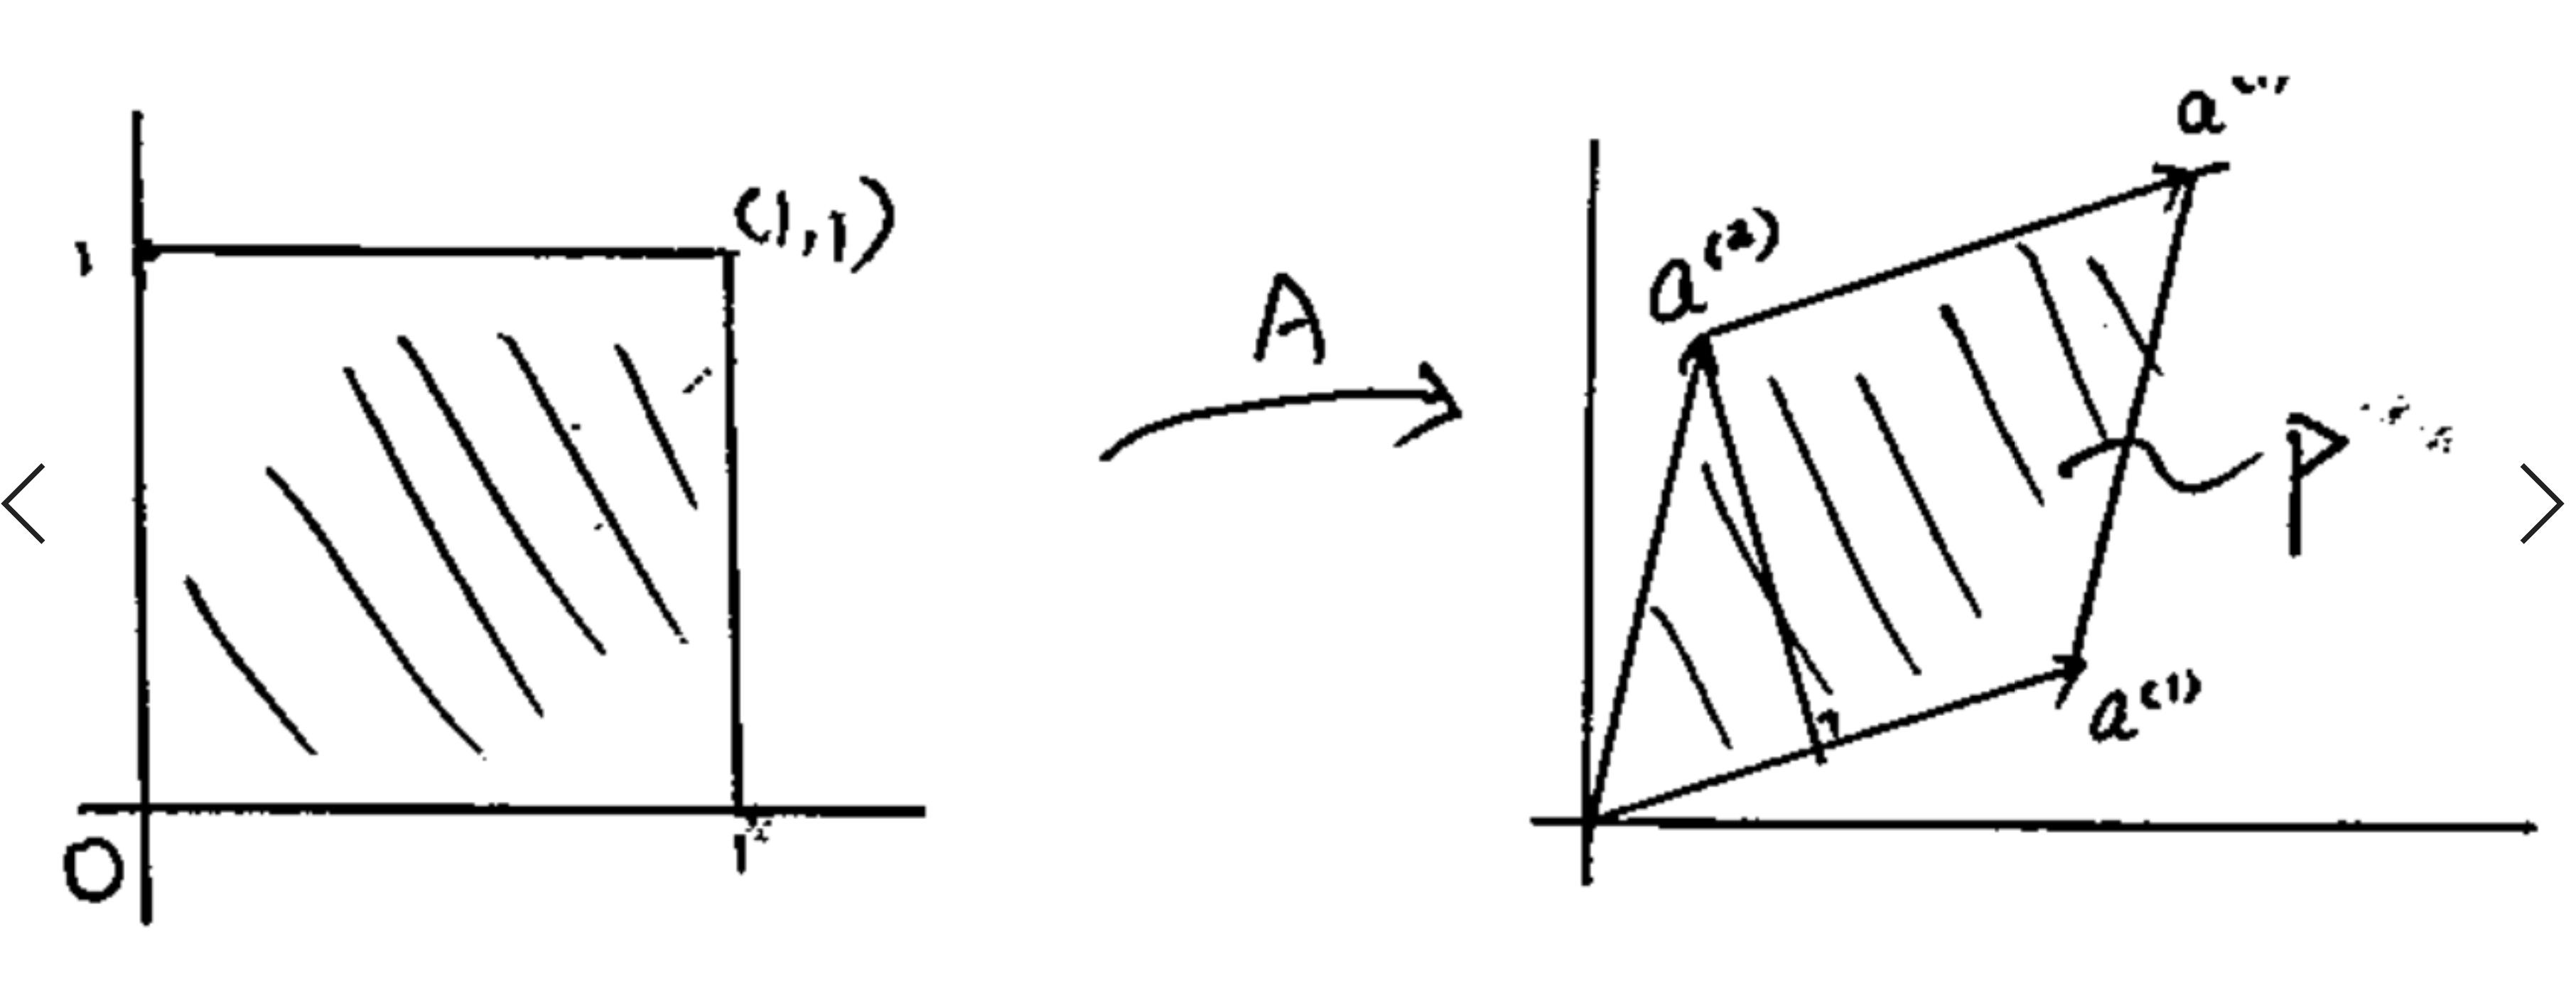
\includegraphics[width=2.1in,height=2.1in]{figures/ch03/figure1.jpg}
	%\caption{This is an inserted JPG graphic} 
	%\label{fig:graph} 
\end{figure}

In this example, the set $\cal{U}$ is mapped to set $P$, via a linear map(multiply by $A$). We find that
$$Vol(P)=\det(A) Vol(\cal{U})$$
That is, $\det(A)$ plays as scaling factor associate with a linear map. 

Recall that if $det(A) = 0$ then $A$ is non-invertible, so if we take a matrix $A$ with $det(A) = 0$ then $P$ will be a line with $Vol(P)=0$.(Recall that it is impossible to invert the map from a lower dimension space back to a higher dimension space).


%Two matrices $A, B \in \reals^{n, n}$ are said to be \textbf{similar} if there exists a nonsingular matrix $P\in \reals^{n,n}$ s.t.:

%\begin{equation*}
%B = P^{-1}AP
%\end{equation*}

%Because there exists vectors $\tilde{x}, \tilde{y}$ s.t.:
%\begin{align}
%x &= P\tilde{x}\\
%y &= P\tilde{y}\\
%P\tilde{y} &= A P\tilde{x}\\
%\tilde{y} &= P^{-1}AP P\tilde{x} = B \tilde{x}
%\end{align}

Assume $A$ is \textbf{diagonalizable}($A$ is similar with a diagonal matrix):
\begin{align*}
A &= U\Lambda U^{-1}\\
|det(A)| &= |det(U\Lambda U^{-1})| \\
&= |det(U)det(\Lambda)det(U^{-1})|\\
&= det(U)det(\Lambda)\frac{1}{det(U)}\\
&= |det(\Lambda)|\\
&= |\prod^n_{i=1}\lambda_i|
\end{align*}

So the determinant of $A$ is zero if there exists an eigenvalue with zero value, and to summarize, $A$ is not invertible if there is an zero eigenvalue. 

%\begin{align*}
%X: N(\mu, \Sigma)\,\,where\,\,(\mu \in \reals^n, \Sigma \in \reals^{n\times n})\\
%P_x(x) = \frac{1}{(2\pi)^{\frac{2}{n}}}\frac{1}{|det\Sigma|^{\frac{1}{2}}}exp[-\frac{1}{2}(x - \mu)^T\Sigma^{-1}(x - \mu)]
%\end{align*}
